\subsubsection{Sourcing Current}
For this second iteration the low power of the shelf linear regulator has been replaced with a custom discrete 12 A adjustable linear regulator based on the LT3080-1 from Linear Technologies.

The first thoughts were to make a fully discrete solution but since the low permitted forward voltage drop of the regulator combined with the big output current and relatively big range made it really challenging to get it stable 
under all operating conditions. For this several hours of LTspice simulations have been performed to in the end move to a design using an off-the-shelf IC as driver for a high power transistor shown in figure \ref{fig:LT3080-1_LinRegSchematic}.

\begin{figure}[h!]
    \centering
    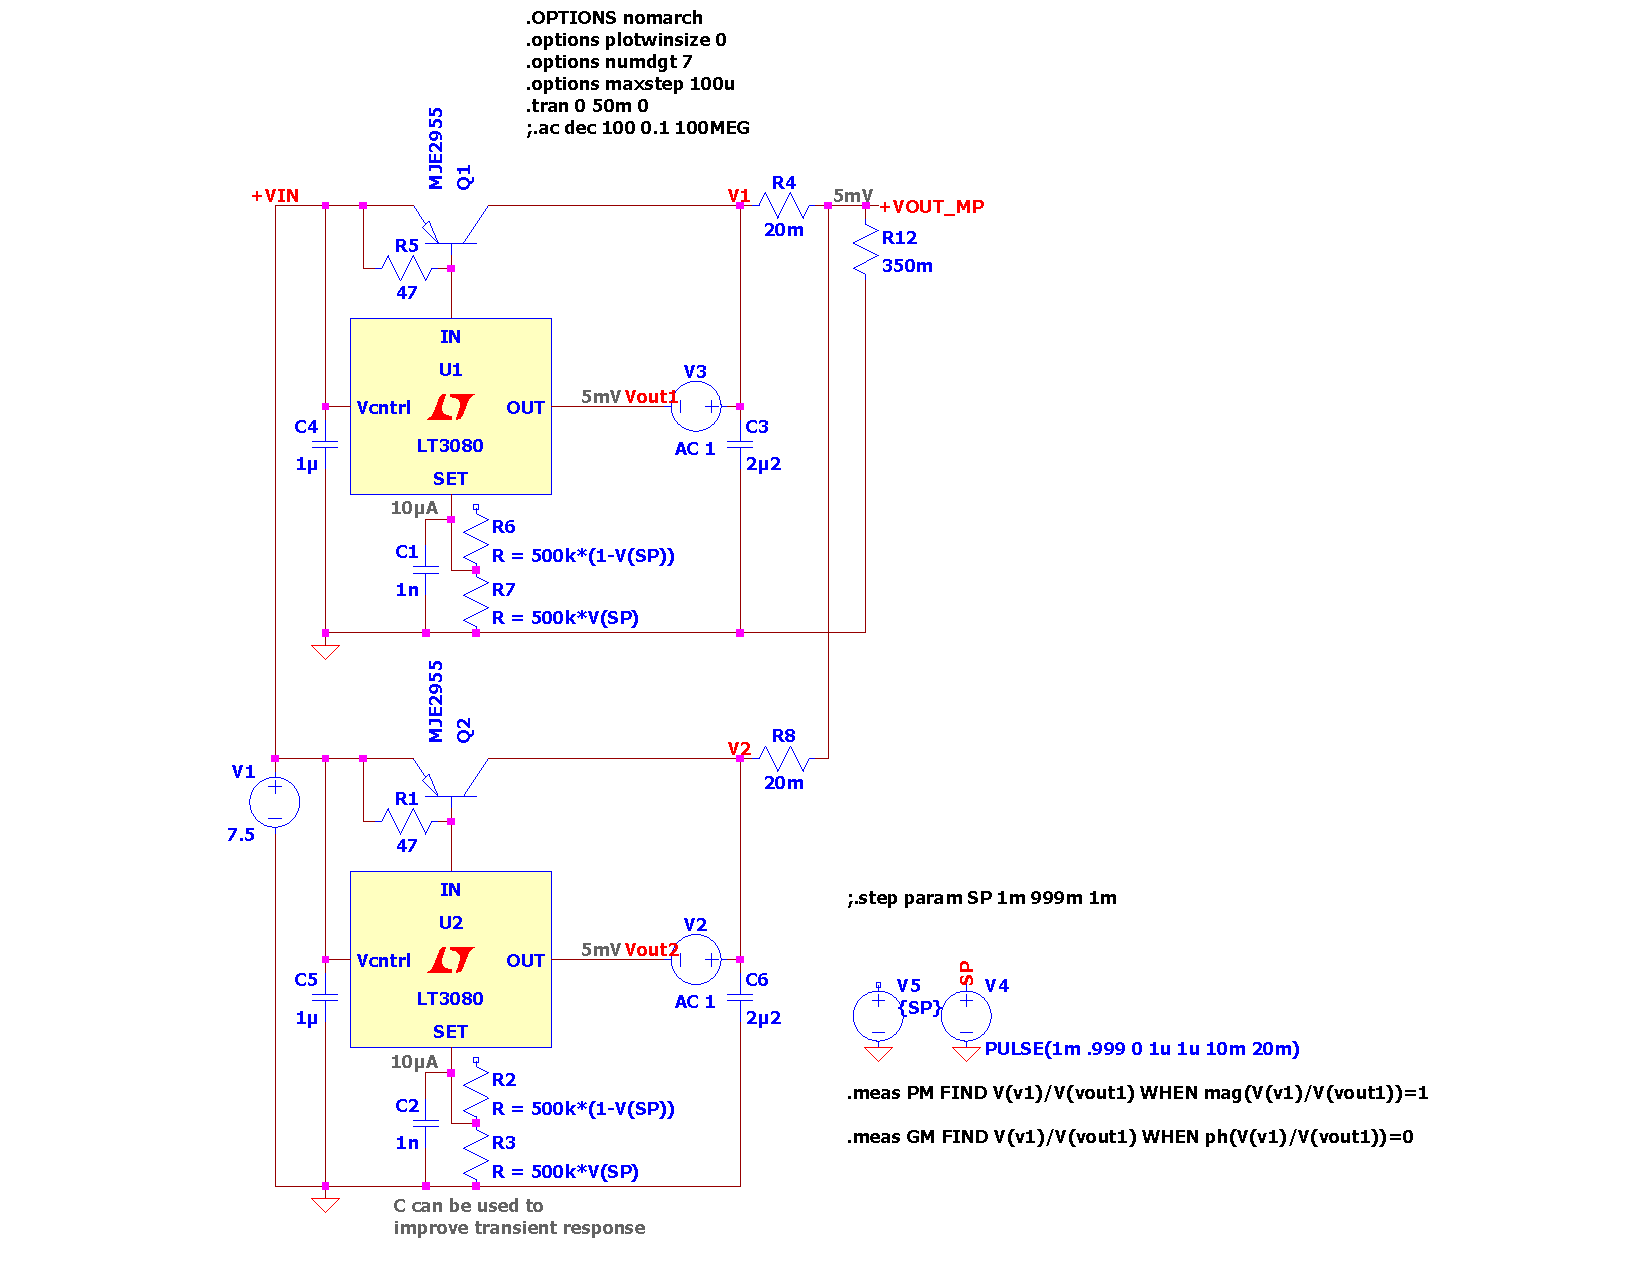
\includegraphics[scale=0.25]{LT3080-1_LinRegSchematic.pdf}
    \caption{12 A linear regulator design based on the LT3080-1}
    \label{fig:LT3080-1_LinRegSchematic}
\end{figure}

The working of the circuit is as follows, xx

Two of these identical circuits are placed in parallel with thier set pins tied together so they are at the same potential. To accomodate proper current sharing two 20 m$\tcohm$ series resistors have been added to give some feedback.
The transient responce of the linear regulator is shown in figure \ref{fig:LT3080-1_LinRegSchematic} and shows that with an input coltage of 7.5 V an output voltage of 0 V up to around 6.9 V can be achieved. The phase margin over setpoint (current) is shown in figure \ref{fig:LT3080-1_Phase-margin_VS_setpoint}. The power dissipation in the main components is shown in figure \ref{fig:LT3080-1_PowerDissipation}.

\begin{figure}[h!]
    \centering
    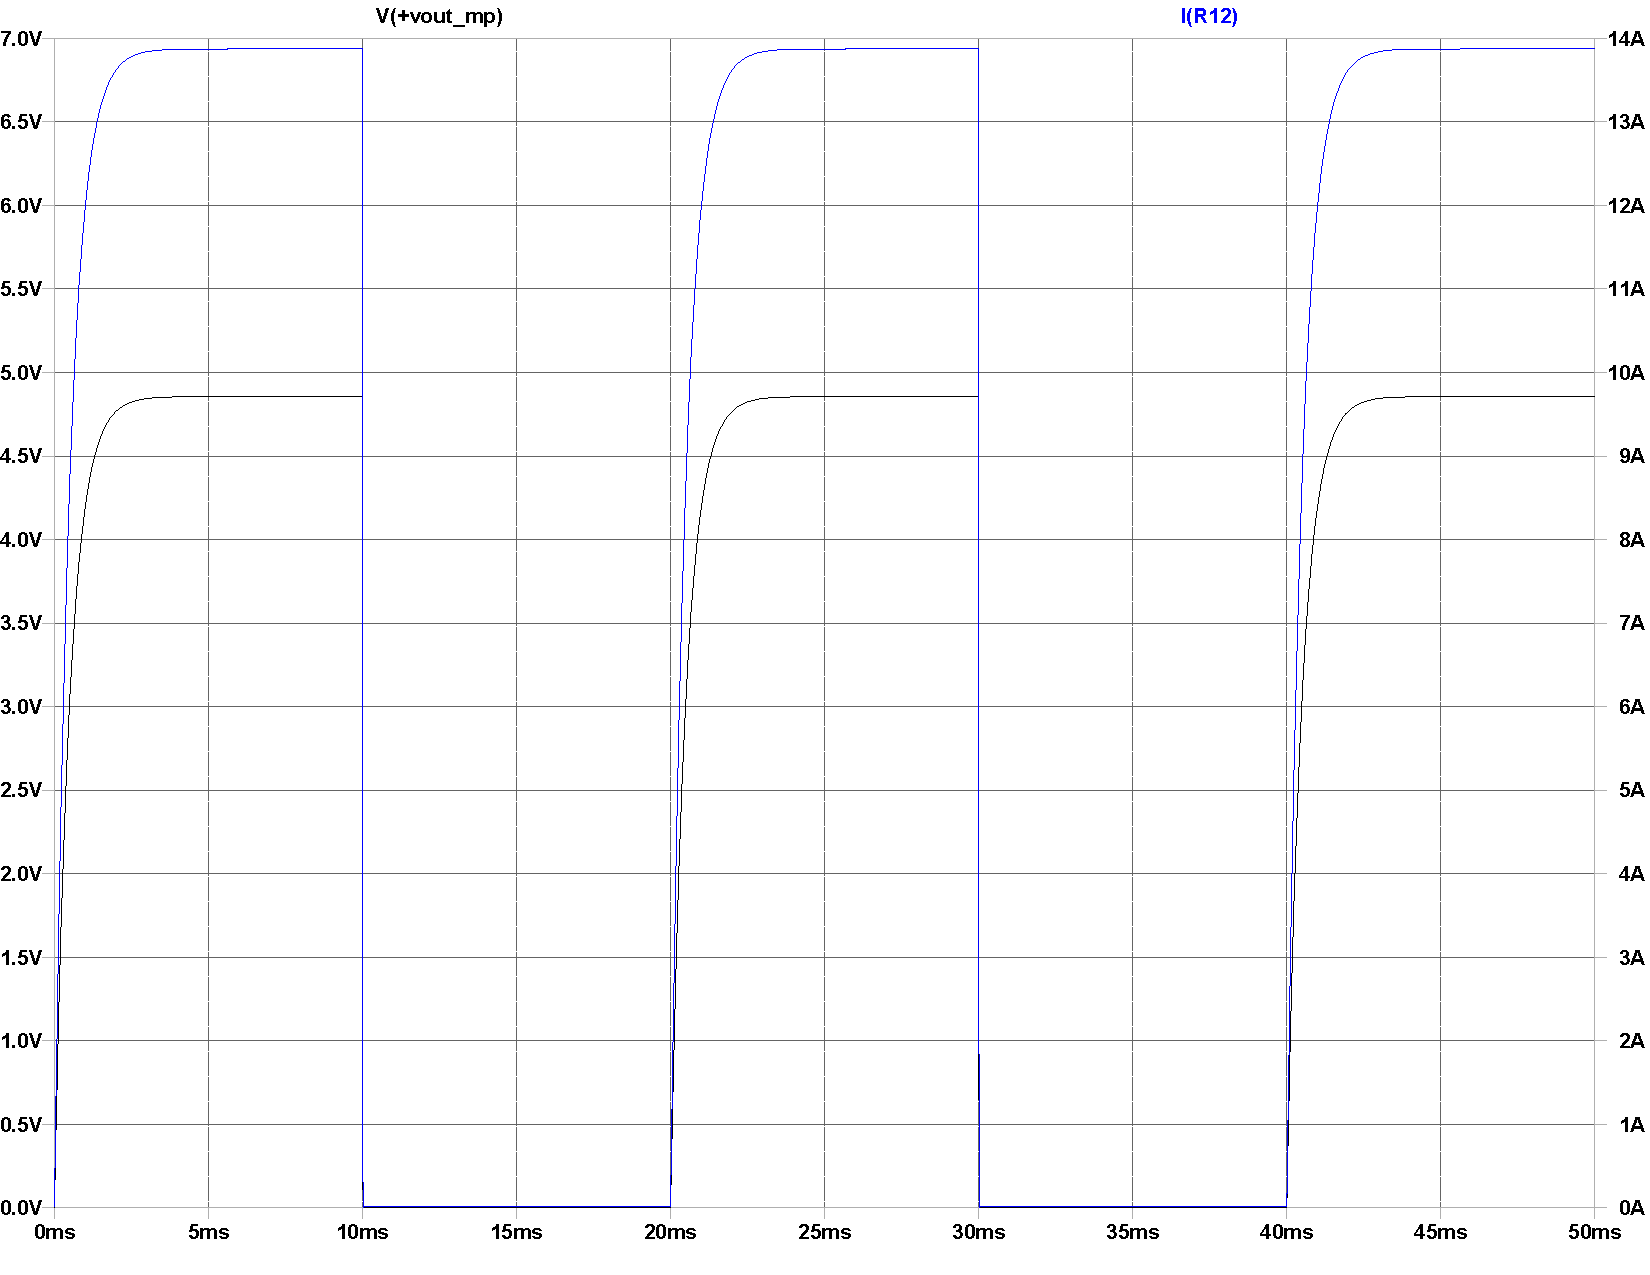
\includegraphics[scale=0.25]{LT3080-1_Transient-response.pdf}
    \caption{12 A linear regulator transient response}
    \label{fig:LT3080-1_Transient-response}
\end{figure}

\begin{figure}[h!]
    \centering
    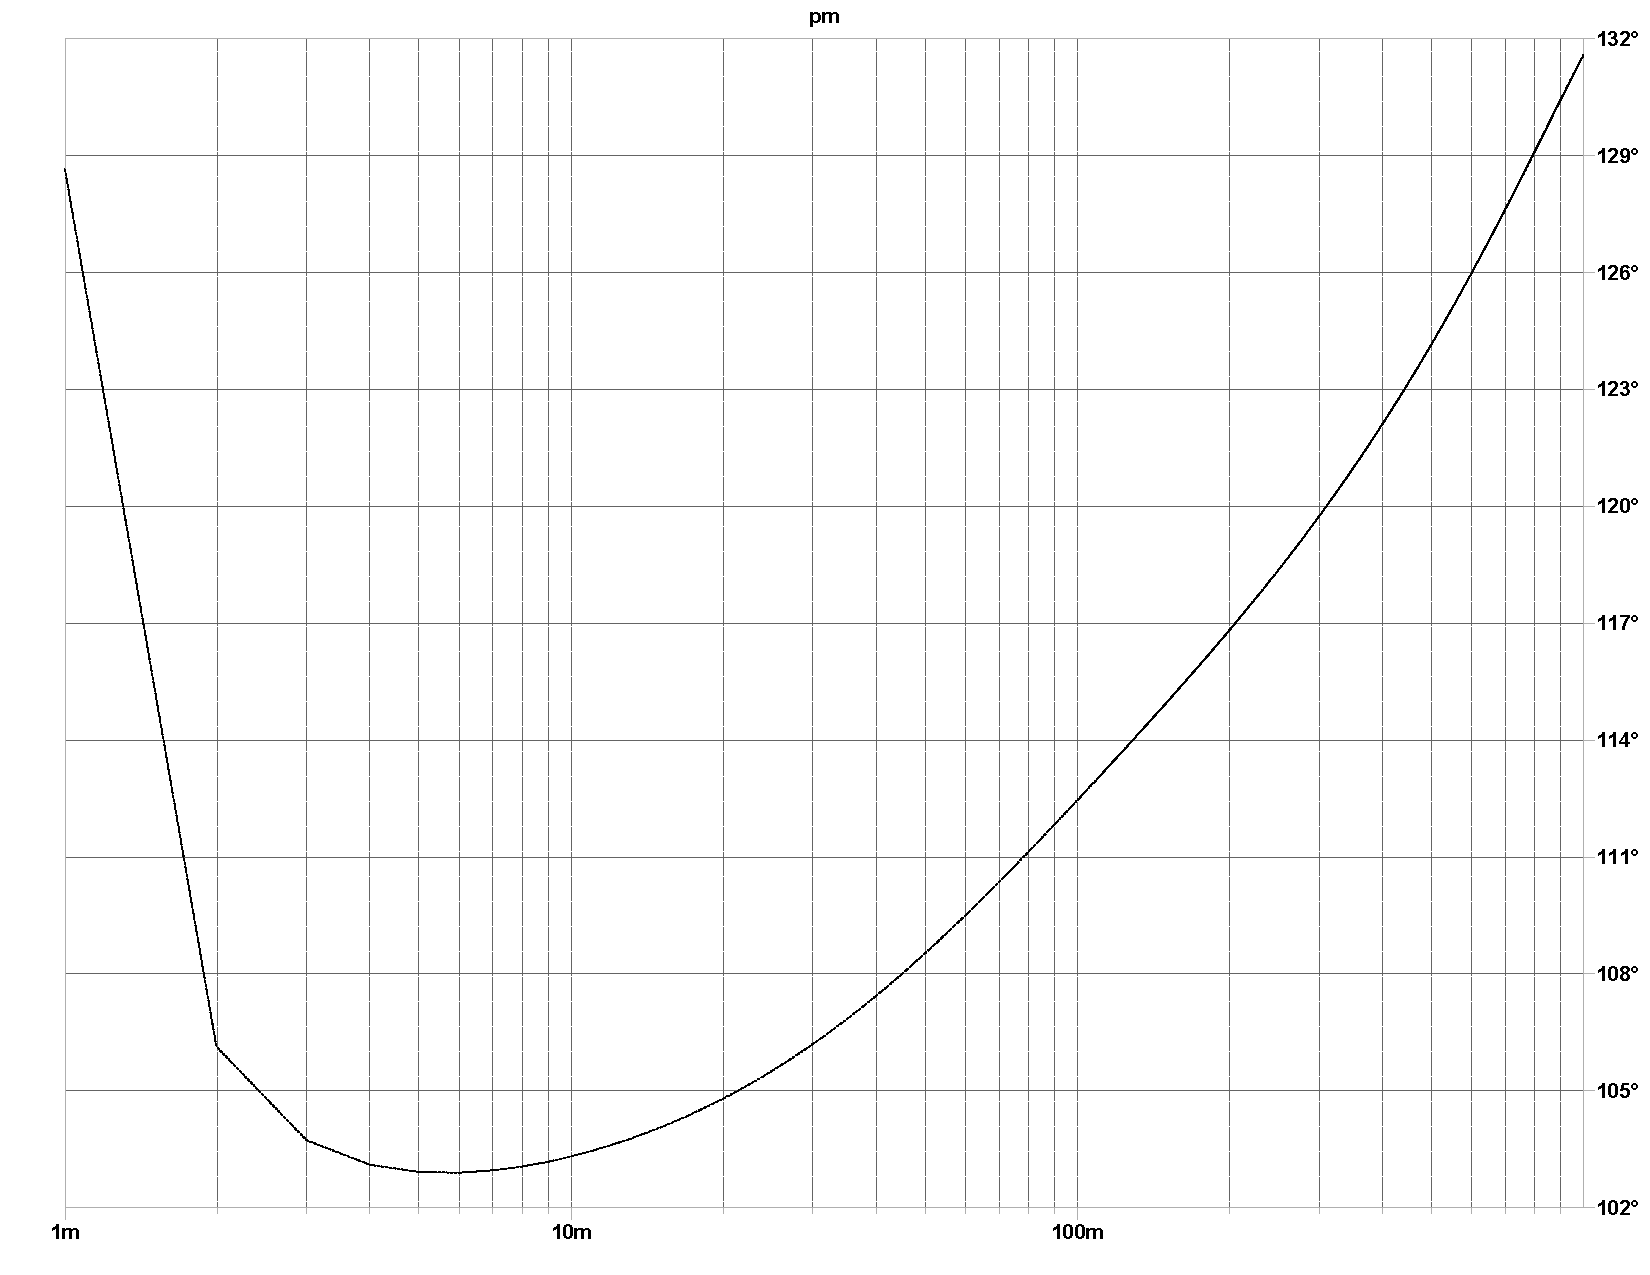
\includegraphics[scale=0.25]{LT3080-1_Phase-margin_VS_setpoint.pdf}
    \caption{12 A linear regulator phase margin vs setpoint (current)}
    \label{fig:LT3080-1_Phase-margin_VS_setpoint}
\end{figure}

\begin{figure}[h!]
    \centering
    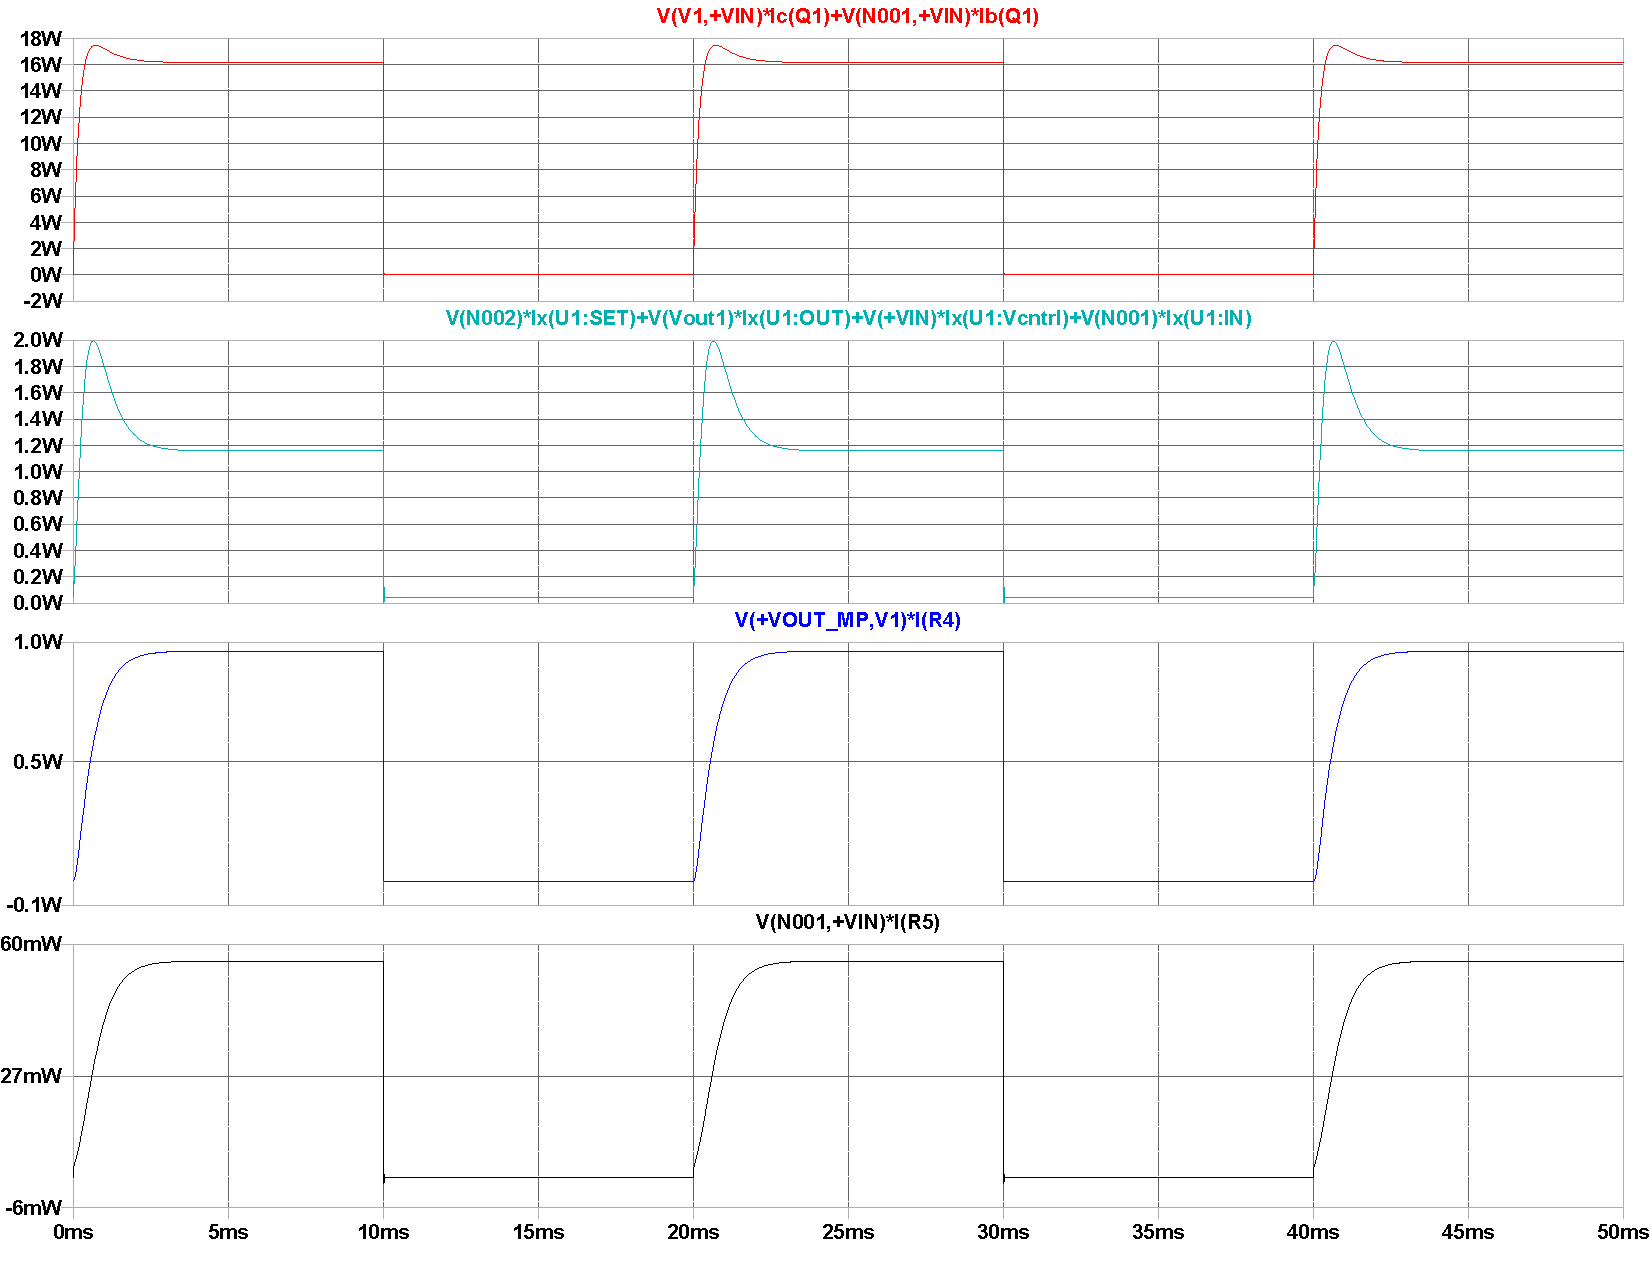
\includegraphics[scale=0.25]{LT3080-1_PowerDissipation.pdf}
    \caption{12 A linear regulator power dissipation}
    \label{fig:LT3080-1_PowerDissipation}
\end{figure}

\subsubsection{Sinking Current}
The current sink is based on an OpAmp driving a N-MOSFET in its linear region controlling the current flowing trough a sense resistor. The OpAmp changes its output so that the voltage across this sense resistor is equal to its setpoint derived from the digital potentiometer. The circuit is shown in \ref{fig:CurrentSinkSchematic}. the resistor directly at the output of the OpAmp is there to limit the phase shift caused by the gate source capacitance of the MOSFET in combination with its parralel RC snubber. Together these components make the current sink stable in its intended operating region.\ref{fig:CurrentSinkSchematic}

\begin{figure}[h!]
    \centering
    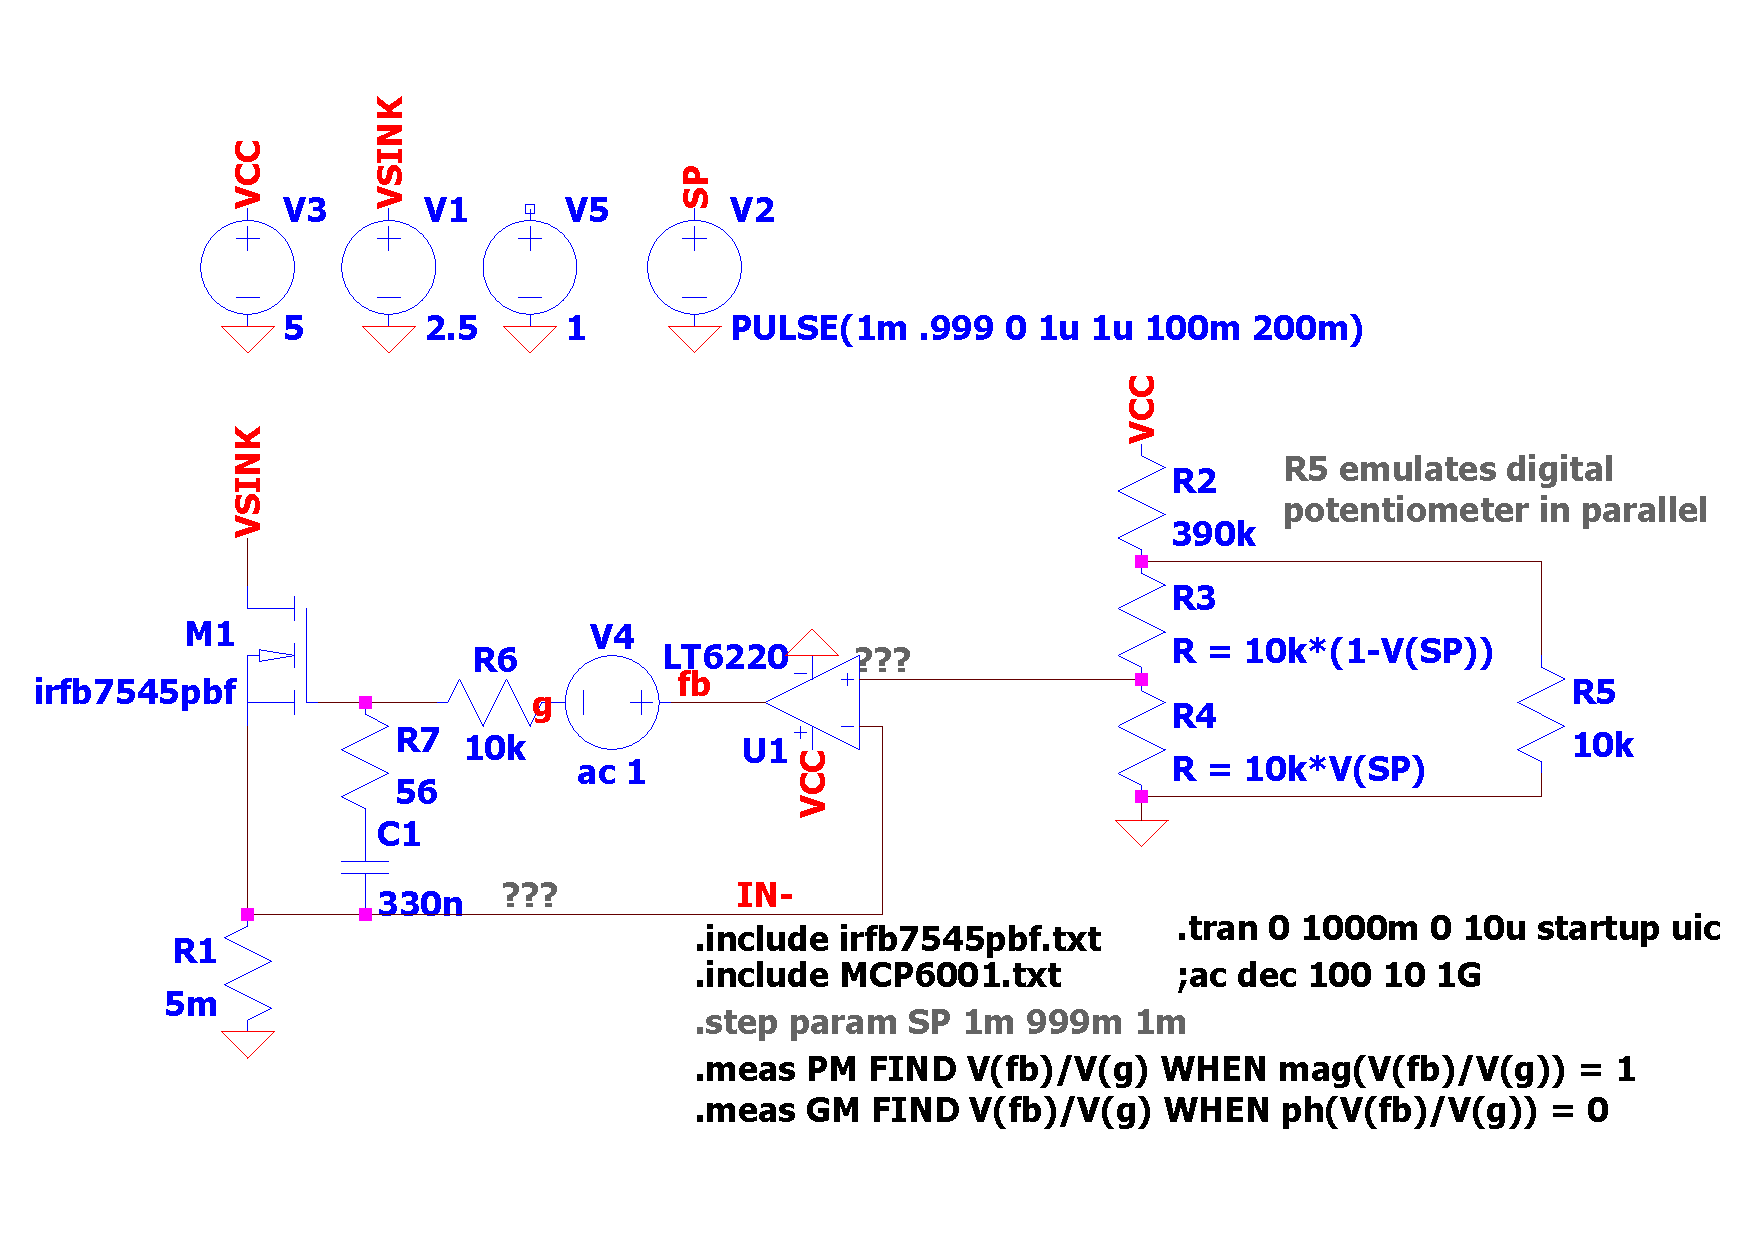
\includegraphics[scale=0.25]{CurrentSinkSchematic.pdf}
    \caption{12 A current sink schematic}
    \label{fig:CurrentSinkSchematic}
\end{figure}

\begin{figure}[h!]
    \centering
    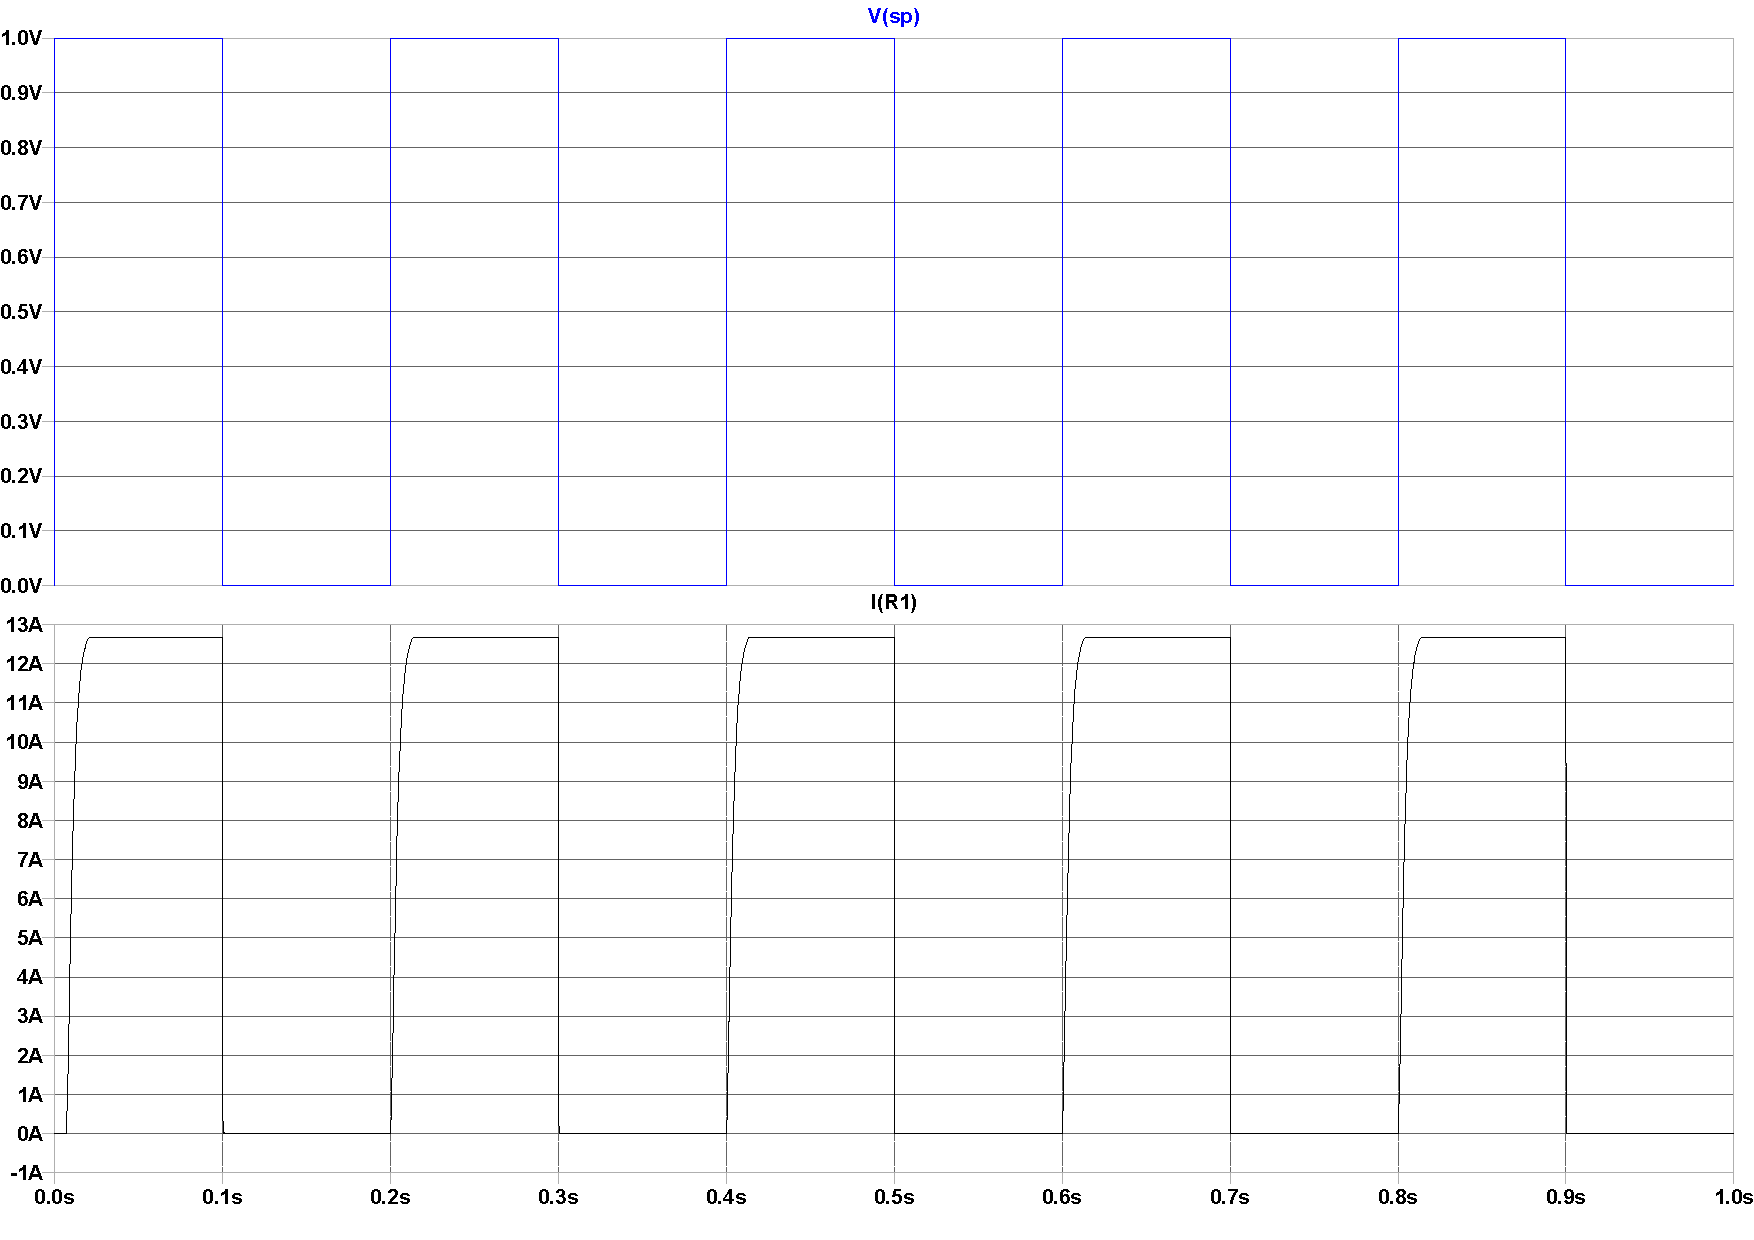
\includegraphics[scale=0.25]{CurrentSinkTransient.pdf}
    \caption{12 A current sink transient responce}
    \label{fig:CurrentSinkTransient}
\end{figure}